% Copyright 2004 by Till Tantau <tantau@users.sourceforge.net>.
%
% In principle, this file can be redistributed and/or modified under
% the terms of the GNU Public License, version 2.
%
% However, this file is supposed to be a template to be modified
% for your own needs. For this reason, if you use this file as a
% template and not specifically distribute it as part of a another
% package/program, I grant the extra permission to freely copy and
% modify this file as you see fit and even to delete this copyright
% notice.

\documentclass{beamer}

\usepackage[utf8]{inputenc}
\usepackage[portuguese]{babel}

% There are many different themes available for Beamer. A comprehensive
% list with examples is given here:
% http://deic.uab.es/~iblanes/beamer_gallery/index_by_theme.html
% You can uncomment the themes below if you would like to use a different
% one:
%\usetheme{AnnArbor}
%\usetheme{Antibes}
%\usetheme{Bergen}
%\usetheme{Berkeley}
%\usetheme{Berlin}
%\usetheme{Boadilla}
%\usetheme{boxes}
%\usetheme{CambridgeUS}
%\usetheme{Copenhagen}
%\usetheme{Darmstadt}
\usetheme{Dresden}     % Legal!
%\usetheme{default}
%\usetheme{Frankfurt}
%\usetheme{Goettingen}
%\usetheme{Hannover}
%\usetheme{Ilmenau}
%\usetheme{JuanLesPins}
%\usetheme{Luebeck}
%\usetheme{Madrid}
%\usetheme{Malmoe}
%\usetheme{Marburg}
%\usetheme{Montpellier}
%\usetheme{PaloAlto}
%\usetheme{Pittsburgh}
%\usetheme{Rochester}
%\usetheme{Singapore}
%\usetheme{Szeged}      % Legal!
%\usetheme{Warsaw}

%\usecolortheme{default}
\usecolortheme{rose}

% Hide navigation controls
\beamertemplatenavigationsymbolsempty

\title{Análise do uso de \textit{feedback} de relevância no Sistema de Integração Lattes-Qualis (SILQ)}

% A subtitle is optional and this may be deleted
% \subtitle{Optional Subtitle}

\author{Carlos Bonetti\inst{1}}
% - Give the names in the same order as the appear in the paper.
% - Use the \inst{?} command only if the authors have different
%   affiliation.

\institute[Universidade Federal de Santa Catarina] % (optional, but mostly needed)
{
  \inst{1}%
  Bacharelando de Ciência da Computação\\
  Departamento de Informática e Estatística\\
  Centro Tecnológico\\
  Universidade Federal de Santa Catarina\\
  \hfill \\
  Orientação: Profa. Dra. Carina F. Dorneles
  %\and
  %\inst{2}%
  %Department of Theoretical Philosophy\\
  %University of Elsewhere
}
% - Use the \inst command only if there are several affiliations.
% - Keep it simple, no one is interested in your street address.

\date{Trabalho de Conclusão de Curso, 2016}
% - Either use conference name or its abbreviation.
% - Not really informative to the audience, more for people (including
%   yourself) who are reading the slides online

% \subject{Theoretical Computer Science}
% This is only inserted into the PDF information catalog. Can be left
% out.

% If you have a file called "university-logo-filename.xxx", where xxx
% is a graphic format that can be processed by latex or pdflatex,
% resp., then you can add a logo as follows:

% \pgfdeclareimage[height=0.5cm]{university-logo}{university-logo-filename}
% \logo{\pgfuseimage{university-logo}}

% Delete this, if you do not want the table of contents to pop up at
% the beginning of each subsection:
%\AtBeginSubsection[]
\AtBeginSection[]
{
  \begin{frame}<beamer>{Sumário}
    %\tableofcontents[currentsection,currentsubsection]
    \tableofcontents[currentsection]
  \end{frame}
}

% ===========================================================================
% Let's get started

\begin{document}

\begin{frame}
  \titlepage
\end{frame}

\begin{frame}{Sumário}
  \tableofcontents
  % You might wish to add the option [pausesections]
\end{frame}

\section{Introdução}

\subsection{Histórico e Justificativa}

\begin{frame}{Histórico e Justificativa}
  \begin{itemize}[<+->]
    \item AGUIAR, Felipe Nedel de; COSTA, Maria Eloísa. \textbf{SILQ - Sistema de Integração Lattes Qualis}. Trabalho de Conclusão de Curso. Florianópolis: Universidade Federal de Santa Catarina, Biblioteca Universitária, 2015.
    \item Qualificação automática de produções científicas através de busca por similaridade textual nos dados Qualis;
    \item \url{http://silq.inf.ufsc.br}
  \end{itemize}
\end{frame}

\begin{frame}
  Fotinhas da primeira versão do SILQ
\end{frame}

\begin{frame}{Lattes}
  \begin{figure}
    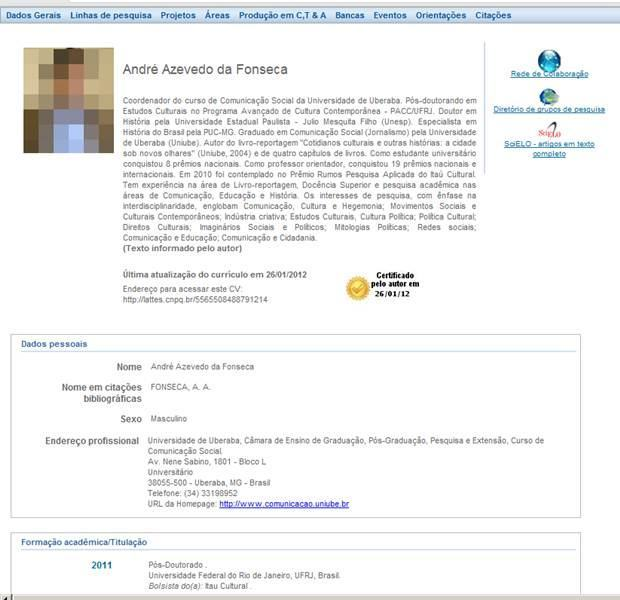
\includegraphics[scale=0.3]{figuras/lattes.jpg}
  \end{figure}
\end{frame}

\begin{frame}{Qualis}
  \begin{figure}
    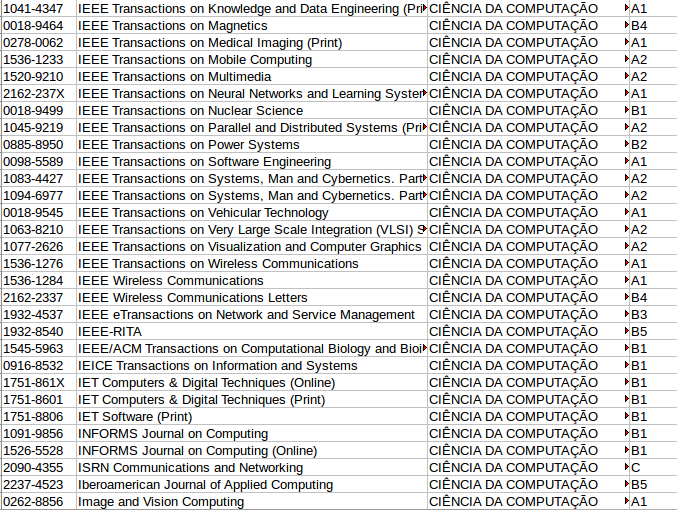
\includegraphics[scale=0.4]{figuras/qualis_exemplo.png}
  \end{figure}
\end{frame}

\begin{frame}
  \begin{block}{Motivação}
    Atualização tecnológica e da base de dados
  \end{block}

  \begin{block}{Hipótese}
    É possível aumentar a taxa de acerto do SILQ utilizando \textit{feedback} de usuários?
  \end{block}
\end{frame}

\subsection{Objetivos}

\begin{frame}{Objetivos}
  \begin{block}{Objetivo geral}
    Analisar o impacto que o uso de feedback de relevância tem na precisão dos resultados de avaliações realizadas pelo SILQ, efetuado sobre uma nova arquitetura da ferramenta que inclui a criação de API de integração com outros sistemas e a atualização da base de dados conforme as novas classificações Qualis.
  \end{block}
\end{frame}

\begin{frame}{Objetivos específicos}
  \begin{enumerate}[<+->]
    \item Reestruturação da arquitetura e banco de dados do SILQ a fim de suportar classificações de eventos e periódicos disponibilizados em um ritmo anual;

    \item Atualização do banco de dados do sistema com as últimas classificações disponibilizadas pelo Qualis (anos 2013 e 2014);

    \item Criação de uma API pública de disponibilização dos serviços do SILQ, via camada de aplicação REST para integração com outros sistemas;
  \end{enumerate}
\end{frame}

\begin{frame}{Objetivos específicos}
  \begin{enumerate}[<+->]
    \setcounter{enumi}{3}

    \item Alterações na interface do sistema incluindo migração de \textit{framework} de interface, inclusão de controles de \textit{feedback}, novos gráficos de acompanhamento de grupos de pesquisa e melhorias gerais de usabilidade;

    \item Propor novos algoritmos de avaliação baseados em similaridade textual e \textit{feedback} de relevância e verificar se a taxa de acerto do sistema foi melhorada com tal ação.
  \end{enumerate}
\end{frame}

\begin{frame}{Procedimentos metodológicos}
  \begin{enumerate}
    \item Atualização tecnológica e arquitetural
      \begin{itemize}[<2->]
        \item Criação da camada \textit{RESTful};
        \item Migração do \textit{framework} de \textit{interface};
        \item Alteração do modelo lógico p/ suporte aos novos dados Qualis;
      \end{itemize}

    \item Inclusão de \textit{feedback} de relevância
      \begin{itemize}[<3->]
          \item Controles de captação de \textit{feedback};
          \item Desenvolvimento do algoritmo de classificação baseado em \textit{feedback};
          \item Avaliação experimental dos algoritmos.
      \end{itemize}
  \end{enumerate}
\end{frame}

\section{Conceitos}

\subsection{Information Retrieval e Data-matching}

\begin{frame}{IR e Data Matching}
  \begin{itemize}
    \item \textit{Information Retrieval} (IR)
    \begin{itemize}
      \item \textit{query}
      \item documentos
    \end{itemize}

    \item \textit{Data-Matching}
    \begin{itemize}
      \item similaridade / dissimilaridade
      \item \textit{threshold}
    \end{itemize}

    \item SILQ: sistema de IR baseado em \textit{data matching}
  \end{itemize}
\end{frame}

\begin{frame}{\textit{n-grams} / \textit{trigrams}}
  \begin{itemize}
    \item n-grams + trigrams
    \item qual trehsold utilizar? qual função de similaridade utilizar?
    \item o sistema apresenta os resultados corretos?
  \end{itemize}
\end{frame}

\begin{frame}{Como o SILQ avalia um currículo Lattes}
  \underline{Artigo \#1} (extraído do Lattes)\\
  \textbf{Título}: Approximate data instance matching: a survey\\
  \textbf{Ano}: 2011\\
  \textbf{Área}: Ciência da Computação\\
  \textbf{Journal}: Knowledge and Information Systems\\
  \textbf{ISSN}: 0219-1377\\

  \hfill \\
  \underline{Artigo \#2} (extraído do Lattes)\\
  ...
\end{frame}

\begin{frame}{Como o SILQ avalia um currículo Lattes}
  \underline{Artigo \#1}\\
  \textbf{Título}: Approximate data instance matching: a survey\\
  \textbf{Ano}: 2011\\
  \textbf{Área}: Ciência da Computação\\
  \textbf{Journal}: Knowledge and Information Systems\\
  \textbf{ISSN}: 0219-1377\\

  \hfill \\
  query: (ISSN, ano, área)\\
  $q_A = (\texttt{0219-1377}, \texttt{2011}, \texttt{Ciência da Computação})$
\end{frame}

\begin{frame}
  $q_A = (\texttt{0219-1377}, \texttt{2011}, \texttt{Ciência da Computação})$

  \pause
  \footnotesize
  \begin{table}
    \begin{tabular}{ c | c | c | c }
      \textbf{Conceito} & \textbf{Ano} & \textbf{ISSN} & \textbf{Título}\\
      \hline \hline

      A2 & \textbf{2011} & 0219-1377 & Knowledge and Information Systems (Print)\\
      A2 & 2012 & 0219-1377 & Knowledge and Information Systems (Print)\\
      B1 & 2014 & 0219-1377 & Knowledge and Information Systems (Print)\\
      A2 & 2010 & 0219-1377 & Knowledge and Information Systems (Print)\\
    \end{tabular}
    \caption{Resultados retornados pelo SILQ para a query $q_A$}
  \end{table}

  \pause
  \normalsize
  \textbf{Resultado}\\
  Artigo \#1 recebe o conceito A2
\end{frame}

\begin{frame}{Como o SILQ avalia um currículo Lattes}
  \underline{Trabalho \#1} (extraído do Lattes)\\
  \textbf{Título}: A Strategy for Allowing Meaningful and Comparable Scores in Approximate Matching\\
  \textbf{Ano}: 2007\\
  \textbf{Área}: Ciência da Computação\\
  \textbf{Evento}: Conference on Information and Knowledge Management (CIKM)\\

  \pause
  \hfill \\
  query: (título do evento, ano, área)\\
  $q_T$ = (\texttt{Conference on Information and Knowledge Management (CIKM)}", \texttt{2007}, \texttt{Ciência da Computação})
\end{frame}

\begin{frame}
  $q_T$ = (\texttt{Conference on Information and Knowledge Management (CIKM)}", \texttt{2007}, \texttt{Ciência da Computação})

  \pause
  \footnotesize
  \begin{table}
    \begin{tabular}{ c | c | p{6.5cm} }
      \textbf{Conceito} & \textbf{Similaridade} & \textbf{Título}\\
      \hline \hline

      A1 & 0.71 & International Conference on Information and Knowledge Management\\ \hline
      B4 & 0.64 & International Conference on Information, Process, and Knowledge Management\\
    \end{tabular}
    \caption{Resultados retornados pelo SILQ para a query $q_T$}
  \end{table}

  \pause
  \normalsize
  \textbf{Resultado}\\
  Trabalho \#1 recebe o conceito A1
\end{frame}

\begin{frame}{Métricas e avaliação de sistemas de IR}
  \begin{itemize}
    \item Precisão e revocação
    \item taxa de acerto / exatidão
    \item conjunto de testes
    \item média de rank recíproco
    \item OFF: arquitetura?? (TODO)
  \end{itemize}
\end{frame}

\section{Desenvolvimento}

% Slide: trabalhos futuros citados pelo SILQ 1?

\subsection{Alterações tecnológicas}
% Slide: Extração e inserção dos novos dados Qualis
  % Citar que o banco foi alterado
% Slide: Migração tecnológica
  % Criação do Web Service
  % Alterações no Front End
  % Garantia da qualidade: testes de software

\subsection{Uso de feedback de relevância}

\begin{frame}{Obtenção de feedback}
  \begin{figure}
    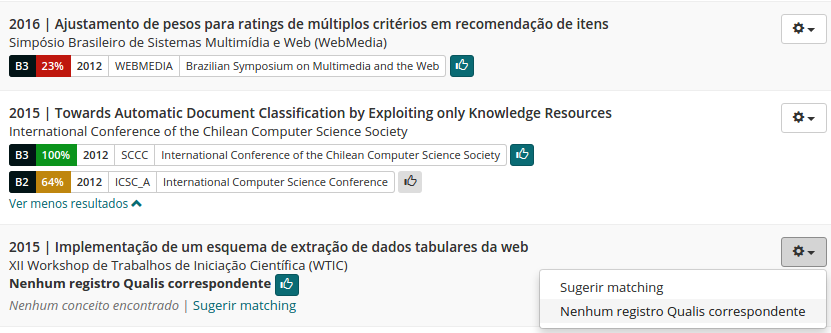
\includegraphics[width=\textwidth]{figuras/feedbacks.png}
    \caption{Controles de feedback da página de resultados de avaliação do SILQ}
  \end{figure}
\end{frame}

\begin{frame}{Algoritmo \texttt{fb(t)}}
  HAL! go ritmo
\end{frame}

\begin{frame}{Algoritmo \texttt{query\_aliasing}}
  HAL! go ritmo
\end{frame}

\begin{frame}{Avaliação de \textit{threshold} ideal}
  \begin{figure}
    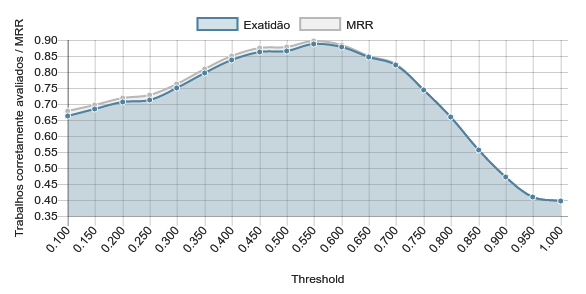
\includegraphics[width=\textwidth]{figuras/avaliacao-threshold.png}
    \caption{Valores de exatidão e MRR para diferentes valores de \textit{threshold} utilizando o método \textit{trigram}}
  \end{figure}
\end{frame}

\begin{frame}{Exatidão dos algoritmos propostos}
  \begin{table}
    \begin{tabular}{ c | c }
      \textbf{Algoritmo} & \textbf{Exatidão} \\
      \hline \hline
      \textit{trgm} & 88.667\% \\
      \textit{trgm + fb(1.00)} & 89.667\% \\
      \textit{trgm + fb(0.90)} & 90.667\% \\
      \textit{trgm + fb(0.80)} & 92.667\% \\
      \textit{trgm + fb(0.70)} & 92.667\% \\
      \textit{trgm + fb(0.60)} & 91.000\% \\
      \textit{trgm + query\_aliasing} & \textbf{93.333}\%
    \end{tabular}
    \caption{Comparação da exatidão dos diferentes algoritmos testados (utilizando \textit{threshold} de $0.55$)}
  \end{table}
\end{frame}

\begin{frame}
  \begin{figure}
    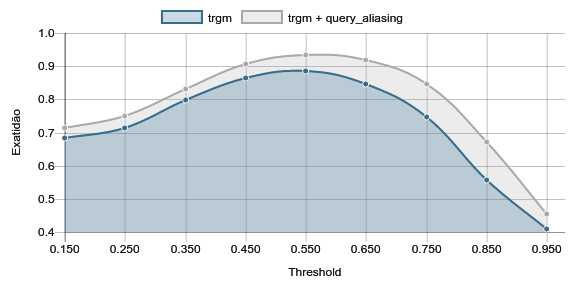
\includegraphics[width=\textwidth]{figuras/avaliacao-algoritmos.png}
    \caption{Comparação da taxa de acerto do algoritmo \textit{trgm} e do \textit{trgm + query\_aliasing} para diferentes \textit{thresholds}}
  \end{figure}
\end{frame}

\section{Conclusões}

\begin{frame}{Conclusões}
  Conclusões.
\end{frame}

\begin{frame}{Trabalhos futuros}
  Trabalhos futuros.
\end{frame}

% All of the following is optional and typically not needed.
\appendix
\section<presentation>*{\appendixname}
\subsection<presentation>*{Encerramento}

\begin{frame}
  \begin{center}
    \large {\usebeamercolor[fg]{structure} Análise do uso de \textit{feedback} de relevância no Sistema de Integração Lattes-Qualis (SILQ)}

    \hfill \break

    \LARGE Dúvidas?

    \hfill \break
    \normalsize Carlos Bonetti \\
    \textit{carlosbonetti.mail@gmail.com}
  \end{center}
\end{frame}

\end{document}
